\section{Effekt och energi}
\textbf{HAREC a.\ref{HAREC.a.1.9}\label{myHAREC.a.1.9}}
\label{effect och energi}
\index{effekt}
\index{energi}

\subsection{Effekt i en sinusformad signal}
\textbf{HAREC a.\ref{HAREC.a.1.9.1}\label{myHAREC.a.1.9.1}}

För beräkning av effekten av en sinusformad signal använder man effektivvärdet
av spänning och ström.

\(U_{eff} = \dfrac{U_{max}}{\sqrt{2}}\) och \(I_{eff} = \dfrac{I_{max}}{\sqrt{2}}\)

\(P = U_{eff} \cdot I_{eff}\)

\subsection{Effektändring uttryckt i dB}
\textbf{HAREC a.\ref{HAREC.a.1.9.2}\label{myHAREC.a.1.9.2}}
\label{decibel}
\index{dB}
\index{dB!effekt}
\index{effekt!dB}

Måtten i det metriska systemet är alldagliga och ingen finner det märkligt att
det t.ex. går tio decimeter på en meter. Däremot är begreppet decibel ovant för
många.

I detta avsnitt förklaras det mycket användbara begreppet decibel. Decibel (dB)
är en tiondedel av grundenheten Bel (B).

Räkning med decibel grundas på logaritmer, som är ett bekvämt sätt att uttrycka
och behandla talvärden.

\begin{quote}\emph{
Decibel är ett dimensionslöst uttryck för graden av dämpning alternativt
förstärkning.
}\end{quote}

\emph{Effektdämpning} är följden av att vissa komponenter bromsar elektrisk ström. Den
bromsande faktorn kan vara en resistans R, induktans L, kapacitans C eller
sammansatta nätverk av R, L och C.

\emph{Effektförstärkning} innebär att en transistor, ett elektronrör eller annan s.k.
aktiv komponent kan styra en större elektrisk ström och därmed större effekt än
den själv styrs med. Vad som förorsakar effektförändringarna går vi inte in på i
detta sammanhang, utan byggdelarna betraktas som ''svarta lådor'' med
anslutningsklämmor.

En byggdel med två ingångs- och två utgångsklämmor kallas för ''fyrpol''.

\begin{figure}[th]
\begin{center}
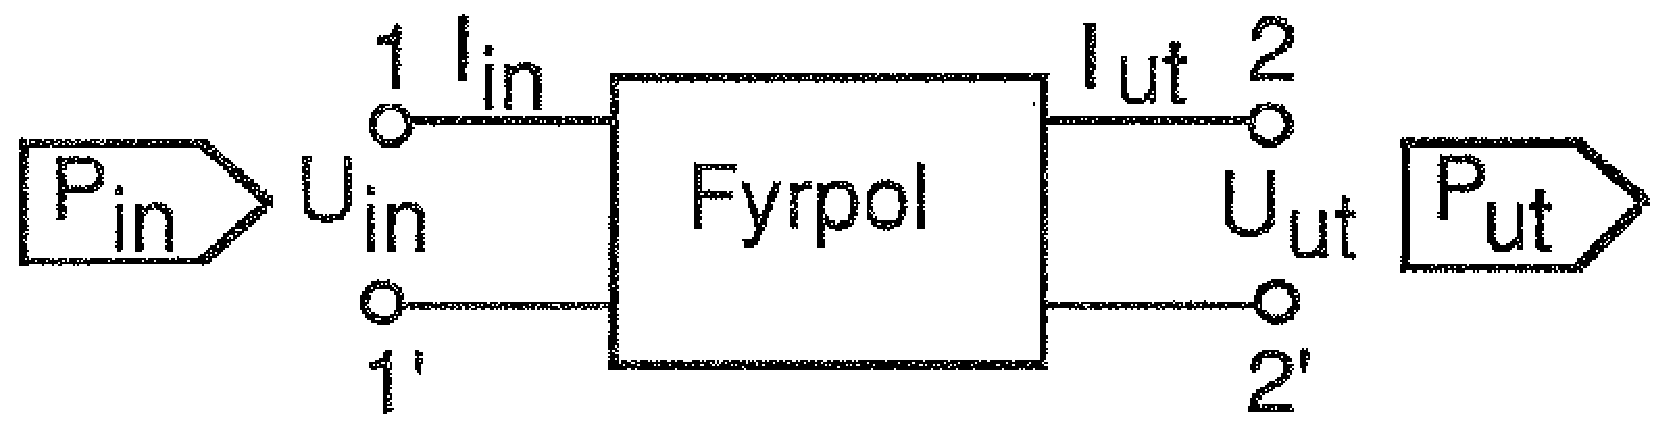
\includegraphics[width=7cm]{images/cropped_pdfs/bild_2_1-32.pdf}
\caption{Effektförhållande}
\label{fig:BildII1-32}
\end{center}
\end{figure}

Antag att den inmatade effekten P är 1~W. Om effekten inte ändras vid passagen
genom fyrpolen, så är även den uttagna effekten 1~W.

\emph{Effektförhållandet} mellan in- och utgångarna är då

\(\dfrac{P_{in}}{P_{ut}} = \dfrac{1\ watt}{1\ watt} = 1 (kvoten = 1)\)

Oförändrad effekt varken dämpas eller förstärks, varför både dämpningen och
förstärkningen har talvärdet 0. Enheten på talvärdet är Bel, dämpningen eller
förstärkningen är således 0~Bel. En tiondel därav är 0~decibel (0~dB).

Omräkning av kvoten av en effektändring till dB görs så, att 10-logaritmen för
kvoten söks och resultatet blir effektändringen uttryckt i Bel (B). Om
resultatet uttrycks i dB, ska Bel-värdet multipliceras med 10.

Logaritmer förklaras i appendix \ref{logaritmer}.

För att förenkla beräkningen av dB-talet divideras det högre effekttalet med det
lägre. Bokstaven a i följande formler betyder antingen förstärkning (+a) eller
dämpning (-a) beroendet på vilket förtecken som sätts.

\(a[B] = \log \dfrac{P_\text{hög}}{P_\text{låg}}\)

\(a[dB] = 10\log \dfrac{P_\text{hög}}{P_\text{låg}}\)

Att addera eller subtrahera värden på en logaritmisk skala, motsvarar att
multiplicera resp. dividera värden på en linjär skala. Huvudskalorna på en
räknesticka är logaritmiska. (Räknestickan är ett enkelt, förut mycket använt
hjälpmedel).

Med hjälp av nomogrammet i bild \ref{ellära-nomogram-db-effekt} kan en \textbf{effektändring}, uttryckt som kvot
(effekterna dividerade med varandra), omvandlas till decibel och omvänt.

\begin{figure}
  \fbox{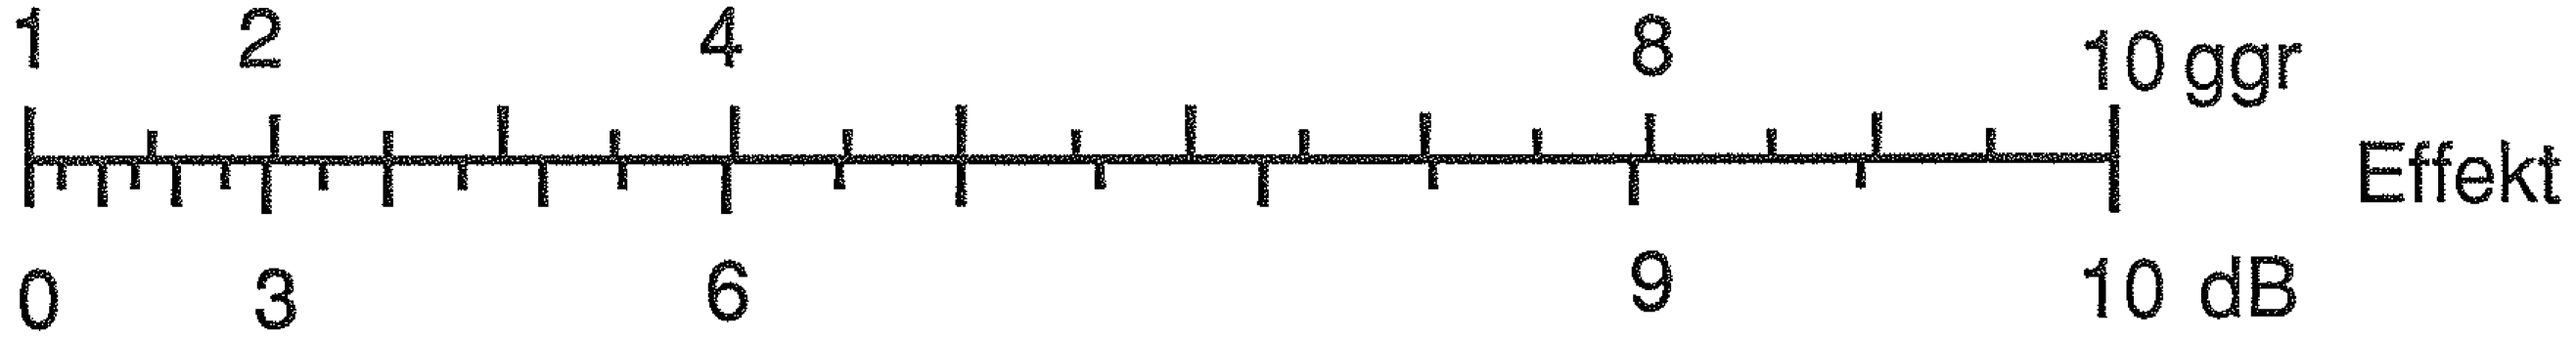
\includegraphics[width=\textwidth]{images/nomogram_db_effekt.png}}
  \caption{Nomogram för omvandling mellan effekt och decibel}
  \label{ellära-nomogram-db-effekt}
\end{figure}

Följande avrundade värden kan utläsas:

\begin{tabular}{rlrlrl}
0 dB & = 1 &  1 dB & =  1,25 & 2 dB = 1,6 \\
3 dB & = 2 &  4 dB & =  2,5  & 5 dB = 3,2 \\
6 dB & = 4 &  7 dB & =  5    & 8 dB = 6,3 \\
9 dB & = 8 & 10 dB & = 10    & 11 dB = 12,5
\end{tabular}

\begin{quote}\emph{
d.v.s. vid ökning fördubblas effekten för var 3:e dB och vid minskning
halveras effekten för var 3:e dB.
}\end{quote}

Om kvoten är en eller flera 10-potenser högre än 10, så kan nomogrammet utökas
enligt följande tabell.

\begin{tabular}{rllr}
Kvot av & Analys             & Skriv            & dB \\
\(P_\text{hög}/P_\text{låg}\) &          &                  &    \\
     1 & 1 har 0 nollor      & \(0 \cdot 10\) = &  0 \\
    10 & 10 har 1 nolla      & \(1 \cdot 10\) = & 10 \\
   100 & 100 har 2 nollor    & \(2 \cdot 10\) = & 20 \\
 1 000 &  1 000 har 3 nollor & \(3 \cdot 10\) = & 30 \\
10 000 & 10 000 har 4 nollor & \(4 \cdot 10\) = & 40
\end{tabular}

\subsection{Strömändring uttryckt i dB}
\index{ström!dB}
\index{dB!ström}

Förhållandet mellan strömmar liksom mellan spänningar kan även uttryckas i dB,
men annorlunda än mellan effekter. En fyrpol med inbördes lika ingångs- och utgångsimpedans är förutsättningen för jämförelse.

Enligt Joules lag är \(P = I^2 \cdot R\) (\(P = U \cdot I\))

således \(\dfrac{P_\text{h{\oe}g}}{P_\text{l{\aa}g}} = \dfrac{I_\text{hög}^2 \cdot R}{I_\text{l{\aa}g}^2 \cdot R}\)

R kan avkortas \emph{om in- och utgångsimpedanserna (resistanserna) är lika}.

En jämförelse uttryckt i dB kan endast göras
under samma förutsättningar; här att impedanserna (resistanserna) är lika,

således \(\dfrac{P_\text{hög}}{P_\text{låg}} = \dfrac{I_\text{hög}^2}{I_\text{låg}^2}\)

Effektförhållandet eller kvadratvärdet på
strömförhållandet kan uttryckas logaritmiskt
i B eller dB

\(a[dB] = 10\log \dfrac{I_\text{hög}^2}{I_\text{låg}^2}\)

Eftersom \(\log x^2 = 2 \cdot \log x\), fås slutligen

\(a[dB] = 20\log \dfrac{I_\text{hög}}{I_\text{låg}}\)

\subsection{Spänningsändring uttryckt i dB}
\index{spänning!dB}
\index{dB!spänning}

Förhållandet mellan spänningar kan uttryckas i dB på ett liknande sätt som med
strömmar.

Enligt Joules lag är \(P = \frac{U^2}{R}\) (\(P = U \cdot I\))

Två effekter kan ställas i förhållande till varandra på följande sätt:

\(\dfrac{P_\text{hög}}{P_\text{låg}}=\dfrac{U_\text{hög}^2 \cdot R}{U_\text{låg}^2 \cdot R}\)

R avkortas och efter omskrivning fås en formel som liknar den för strömmar

\(\dfrac{P_\text{hög}}{P_\text{låg}} = \dfrac{U_\text{hög}^2}{U_\text{låg}^2}\)

\(a[dB] = 20\log \dfrac{U_\text{hög}}{U_\text{låg}}\)

Med nomogrammet i bild \ref{ellära-nomogram-db-spänning} kan kvoten av en ström- eller spänningsändring omvandlas
till decibel och tvärt om.

\begin{figure}
  \fbox{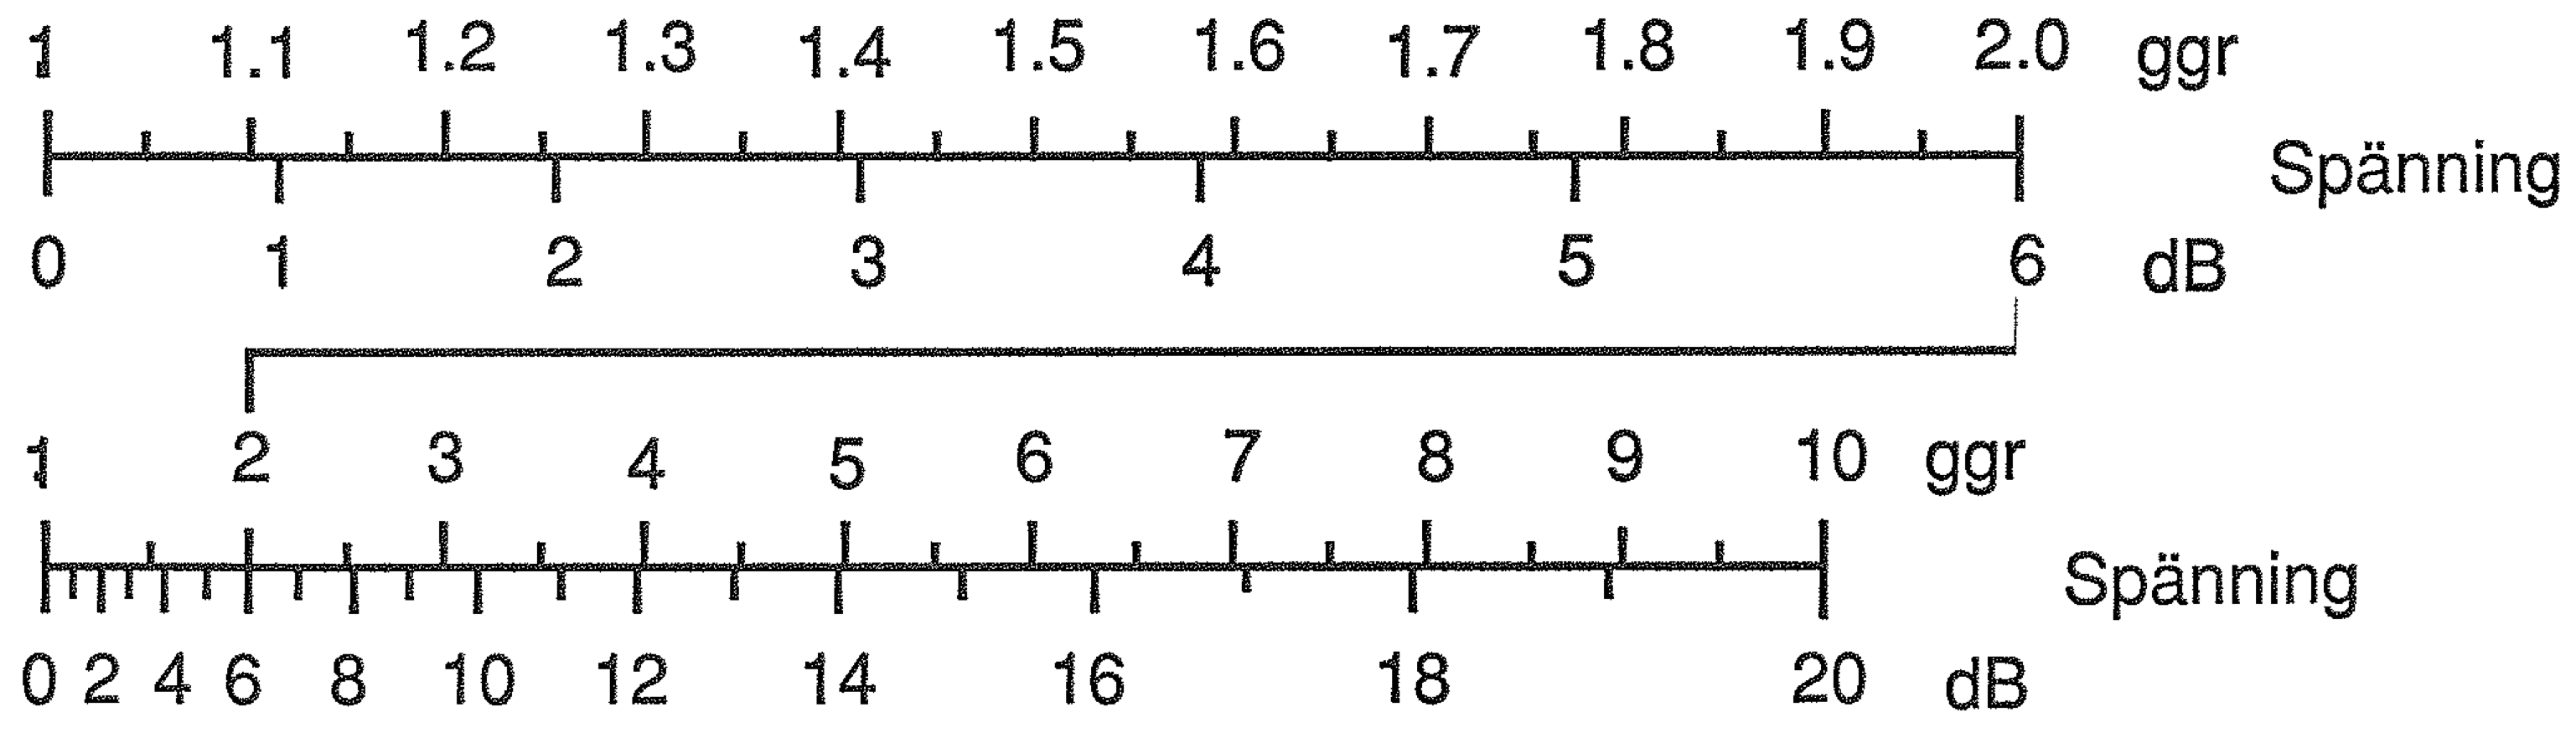
\includegraphics[width=\textwidth]{images/nomogram_db_spanning.png}}
  \caption{Nomogram för omvandling mellan spänning och decibel}
  \label{ellära-nomogram-db-spänning}
\end{figure}

Följande avrundade värden kan utläsas:

\begin{tabular}{rlrlrl}
0 dB & = 1   &  1 dB & = 1,12 &  2 dB = 1,25 \\
3 dB & = 1,4 &  4 dB & = 1,6  &  5 dB = 1,8 \\
6 dB & = 2   &  7 dB & = 2,24 &  8 dB = 2,5 \\
9 dB & = 2,8 & 10 dB & = 3,2  & 11 dB = 3,6
\end{tabular}

\begin{quote}\emph{
d. v. s. vid ökning fördubblas strömmen resp. spänningen för var 6:e dB och att
vid minskning halveras strömmen resp. spänningen för var 6:e dB.
}\end{quote}

Om kvoten är en eller flera 10-potenser högre än 10, så kan nomogrammet utökas
enligt följande tabell.

\begin{tabular}{rllr}
Kvot av & Analys             & Skriv            & dB \\
\(U_\text{hög}/U_\text{låg}\) &          &                  &    \\
\(I_\text{hög}/I_\text{låg}\) &          &                  &    \\
     1 & 1 har 0 nollor      & \(0 \cdot 20\) = &  0 \\
    10 & 10 har 1 nolla      & \(1 \cdot 20\) = & 20 \\
   100 & 100 har 2 nollor    & \(2 \cdot 20\) = & 40 \\
 1 000 &  1 000 har 3 nollor & \(3 \cdot 20\) = & 60 \\
10 000 & 10 000 har 4 nollor & \(4 \cdot 20\) = & 80
\end{tabular}

\section{dB med miniräknare}

När beräkningen av förstärkning eller dämpning uttryckt i dB görs med
miniräknare låter man räknaren sköta hela beräkningen.

Med miniräknare skrivs uttrycken för dB så här:

För effekt \(a[dB] = 10\log \dfrac{P_\text{ut}}{P_\text{in}}\)

För spänning \(a[dB] = 20\log \dfrac{U_\text{ut}}{U_\text{in}}\)

\textbf{Lägg märke till hur värdena ut och in används i ekvationerna.}

Detta gör att man vid beräkningen automatiskt får positiva svar för
förstärkning och negativa svar för dämpning.

\section{Decibel över 1 m W vid 50 \(\Omega\) [dB(m)]}

Det är mycket vanligt att in- och utgångarna i HF-utrustningar utförs
med en impedans av 50~\(\Omega\). För god anpassning väljs då koaxialkablarna
mellan apparaterna med en karaktäristisk impedans av 50~\(\Omega\).

\emph{Det har utbildats en praxis, att referensvärdet vid jämförelse
	av signalnivåer i radiosystem ska vara en milliwatt (1~mW)
	utvecklad i en belastning med impedansen 50~\(\Omega\).}

Signalnivåer över belastningen 50~\(\Omega\) kan uttryckas i dB(m), där (m)
står för milliwatt, varvid referenseffekten 1~mW är 0~dB(m) vid 50~\(\Omega\).

Det spänningsfall som bildas över belastningen 50~\(\Omega\) vid effektnivån
0~dB( m) är

\[U = \sqrt{P\cdot R} = 1\cdot 10^{-3} \cdot 50 \approx 0.224 \text{ V}\]

Den ström som flyter genom belastningen 50~\(\Omega\) vid effektnivån 0~dB(m)
är

\[
I = \sqrt{P}{R} = \sqrt{1\cdot 10^{-3}}{50} = 0.0045 \text{ A} = 4.5 \text{ mA}
\]

Strömmen 4.5~mA genom belastningen 50~\(\Omega\) motsvarar således 0~dB(m).

Varje annan effekt, spänningsfall och ström som uppstår vid en
belastning av 50 \(\Omega\) kan jämföras med respektive referensvärden 1~mW,
0.22~V och 4.5~mA.

\emph{dB(m) är ett absolut och logaritmiskt mått.}

Effekt

\begin{gather*}
	a [dB(m)] = 10 \log\frac{P_{[50 \Omega]}}{1[mW_{50 \Omega}]} \\
	P_{50} = 1 [mW] \cdot 10^{\frac{a}{10}}
\end{gather*}

Ström

\begin{gather*}
	0 dB(m) = 4.47 mA_{50} \\
	a [dB(m)] = 20 \log\frac{I_{50}}{4.47}
\end{gather*}

Spänning

\begin{gather*}
	0 dB(m) = 0.223 V_{50} \\
	a [dB(m)] = 20 \log\frac{U_{50}}{0.223} \\
	U_{50} = 0.223 \cdot 10^{\frac{a}{20}}
\end{gather*}

\section{Sambandet mellan spänning över 50 \(\Omega\) och dB(m)}
\begin{tabular}{l|lp{1cm}l|l}
	dB(m) & V & & dB(m) & V \\
	\cline{1-2} \cline{4-5}
	-40 & 0.00224 & & & \\
	-30 & 0.00707 & & & \\
	-20 & 0.0224  & & & \\
	-10 & 0.0707  & & & \\
	0   & 0.224   & & & \\
	1   & 0.251   & & 11 & 0.793 \\
	2   & 0.282   & & 12 & 0.890 \\
	3   & 0.316   & & 13 & 0.999 \\
	4   & 0.354   & & 14 & 1.121 \\
	5   & 0.398   & & 15 & 1.257 \\
	6   & 0.446   & & 16 & 1.411 \\
	7   & 0.501   & & 17 & 1.583 \\
	8   & 0.562   & & 18 & 1.776 \\
	9   & 0.630   & & 19 & 1.993 \\
	10  & 0.707   & & 20 & 2.236 \\
\end{tabular}

\emph{dB(W) är ett annat absolut mått.}

Effektnivåer över en belastning kan också uttryckas i dB(W), där (W)
står för watt.  Referenseffekten är då 1~W, d.v.s. 0~dB(W).  Liksom med
dB(m) anges impedansen i den belastning, som effekten utvecklas över.

\subsection{Ändring uttryckt i dB vid förstärkande eller dämpande anordningar kopplade i serie}
\textbf{HAREC a.\ref{HAREC.a.1.9.3}\label{myHAREC.a.1.9.3}}

Ett räkneexempel på effektändringar:
Fråga:
Vi har en enkel sändaranläggning med ett drivsteg med en in effekt av 10~W.
Drivsteget förstärker med 6~dB. Vidare har vi ett effektslutsteg som förstärker
med 10~dB. Antennkabeln dämpar med 1~dB.

Med vilken effekt matas själva antennen?

Svar: (två sätt att lösa uppgiften)
\begin{enumerate}
\item Drivsteget förstärker fyra gånger, slutsteget förstärker tio gånger och
kabeln dämpar \(1/1,25 = 0,8\) gånger. Antennen matas då med
\(10 \cdot 4 \cdot 10 \cdot 0,8 = 320\ W\).
\item Drivstegets 6~dB plus slutstegets 10~dB minus antennkabelns 1~dB = 15~dB.
15~dB är \(10 + 5\ dB\) d.v.s. \(10 \cdot 3,2 = 32\ ggr\). Antennen matas med
\(10\ W \cdot 32 = 320\ W\).
\end{enumerate}

\subsection{Impedansanpassning}
\textbf{HAREC a.\ref{HAREC.a.1.9.4}\label{myHAREC.a.1.9.4}}
\index{impedansanpassning}
\index{impedans!anpassning}

Impedansanpassning är av stor betydelse inom kommunikationstekniken.
Normalt vill man nämligen överföra mesta möjliga effekt från energikällan
(t.ex. sändaren) till förbrukaren (t.ex. antennen).

Varje spänningskälla har en inre resistans \(R_i\). Det innebär som först att
källan inte kan avge oändligt stor ström. För att förenkla det hela antar vi nu
att en sändare med den inre resistansen \(R_i\) ansluts direkt till en antenn
med resistansen \(R_a\).

Målet med anpassningen är att finna det optimala förhållandet mellan
sändarresistansen och antennresistansen för att kunna överföra maximal effekt.
Vi har de två ytterlighetsfallen obelastad sändare respektive kortsluten
sändare. Sändarens elektromotoriska kraft (EMK) betecknas som \(E\ [V]\) och
sändarens utspänning som \(U\ [V]\).

Fall 1.
En obelastad sändare avger ingen ström när ingen antenn eller en med oändligt
stor resistans har anslutits.
Alltså vid obelastad sändare:

\(
\begin{array}{lllll}
R_a = \infty & & I = 0 & & U = E
\end{array}
\)

Fall 2.
När sändarutgången är kortsluten, d.v.s. belastningen (antennresistansen) är
noll ohm, avger sändaren en ström som beror av EMK och inre resistans. Eftersom
sändarutgången är kortsluten är utspänningen \(U\) noll.
Alltså vid kortsluten sändare:

\(
\begin{array}{lllll}
R_a = 0 & & I = \dfrac{E}{R_i} & & U = O
\end{array}
\)

I båda ytterlighetsfallen är den effekt som omsätts i \(R_a\) lika med noll.
För att få ut någon effekt måste man alltså söka ett värde på \(R_a\) som
ligger mellan ytterlighetsvärdena.

Enligt formeln för spänningsdelare är utspänningen

\(U = E \cdot \dfrac{R_a}{R_a+R_i}\)

Formeln för uteffektens effektivvärde är

\(P_{ut} = \dfrac{U^2}{R_a}\)

Efter insättning får man

\(P_{ut} = \dfrac{E^2 \cdot R_a}{(R_a + R_i)^2}\)

För att finna det optimala förhållandet mellan \(R_i\) och \(R_a\), d.v.s. när
\(R_a\) tar upp maximal effekt, måste man differentiera formeln med \(d\ P_a/d\ R_a\), men vi hoppar över denna utflykt i matematiken.

I stället konstaterar vi helt enkelt att \emph{maximal effektöverföring sker när
\(R_i = R_a\)}.

\subsection{Förhållandet mellan in- och uteffekt uttryckt som procent verkningsgrad}
\textbf{HAREC a.\ref{HAREC.a.1.9.5}\label{myHAREC.a.1.9.5}}
\index{verkningsgrad}

Antag att en antennkabel har en effektförlust av 1~dB. Det innebär en
effektdämpning av 1,25 gånger, d.v.s. 0,8. Nu matar vi in 10~W i kabeln och får
alltså ut 8~W. Hur stor verkningsgrad har kabeln uttryckt i \% ?
Lösning:

\(\eta = \frac{8}{10} \cdot 100 = 80\ \%\)

\subsection{Toppvärdeseffekt P.E.P.}
\textbf{HAREC a.\ref{HAREC.a.1.9.6}\label{myHAREC.a.1.9.6}}
\index{toppvärdeseffekt}
\index{effekt!toppvärdes}
\index{P.E.P.}
\index{effekt!P.E.P.}

Uteffekten från en sändare kan mätas över en konstlast (dummy load). En
konstlast är en resistor som kan omsätta sändarens hela effekt till värme. Med
HF-mätprob och en detektordiod eller en HF-voltmeter kan man mäta
effektivvärdet på spänningen över konstlasten och beräkna uteffekten med
formeln

\(P_{ut} = \frac{U^2}{R}\)

U = HF-spänningens effektivvärde
R = resistansen i konstlasten

På grund av utsignalens karaktär kan man inte mäta effektivvärdet av uteffekten
från SSB-sändare. Med oscilloskop kan man emellertid mäta utspänningen på den
största modulationstoppen.

Med detta toppvärde kan man beräkna spänningen över konstlasten.

Uteffekten definierad som P.E.P. (Peak Envelope Power) är ''den medeleffekt som
matas in i en antennmatarledning under det högsta effektvärdet inom en
frekvenscykel och mätt under normal drift''.

\(P.E.P. = \dfrac{\hat{u}^2}{R}\)

där \(\hat{u}\) är momentanspänningen på den största modulationstoppen.
